% !TeX spellcheck = da_DK
\subsection{Accelerometer}
\subsubsection{Teori og design}
Teorien bag accelerometret ADXL335 ses i afsnit \ref{Subsec:AccTeori} på side \pageref{Subsec:AccTeori}. Designet kan ses i bilag \ref{Bilag:Pilotforsoeg} på side \pageref{Bilag:Pilotforsoeg}, dog med en ændring af den ene kondensator. I pilotforsøget blev det påvist, at signalet i dette tilfælde ligger mellem $0-25Hz$, og derfor skal der nu benyttes en ny kondensator.\cite{Devices2009}:
\begin{equation}
\text{Båndbredde} = \dfrac{5\mu F}{C} \Rightarrow  C = \dfrac{5\mu F}{\text{Båndbredde}}
\end{equation}
Der vælges en båndbredte på $25$Hz, hvilket gør, at C bliver $0.2\mu$F.  

\subsubsection{Simulering}
Ifølge tolerancerne for accelerometret beskrevet i afsnit \ref{OpsamlingsAfs} på side \pageref{OpsamlingsAfs} skal der testes for, hvorledes accelerometret overholder kravet om, at der maks må være en $5\%$ afvigelse i detektionen af hældningsgrad. \\
Der findes ikke et accelerometer i programmet LTspice, hvorfor accelerometeret er symboliseret med en sinuskurve. Dets DC svarer til strømforsyningen $5.5$V fratrukket offsettet for accelerometeret ved $0$g påvirkning, som er $1.6325$V. Derudover angives en amplitude svarende til den maksimale sensitivitet på $0.3313$V. Simuleringen ses på \figref{fig:acc_simulering} og resultatet ses på \figref{fig:acc_simulering_resultat}.
\begin{figure}[H]
	\centering
	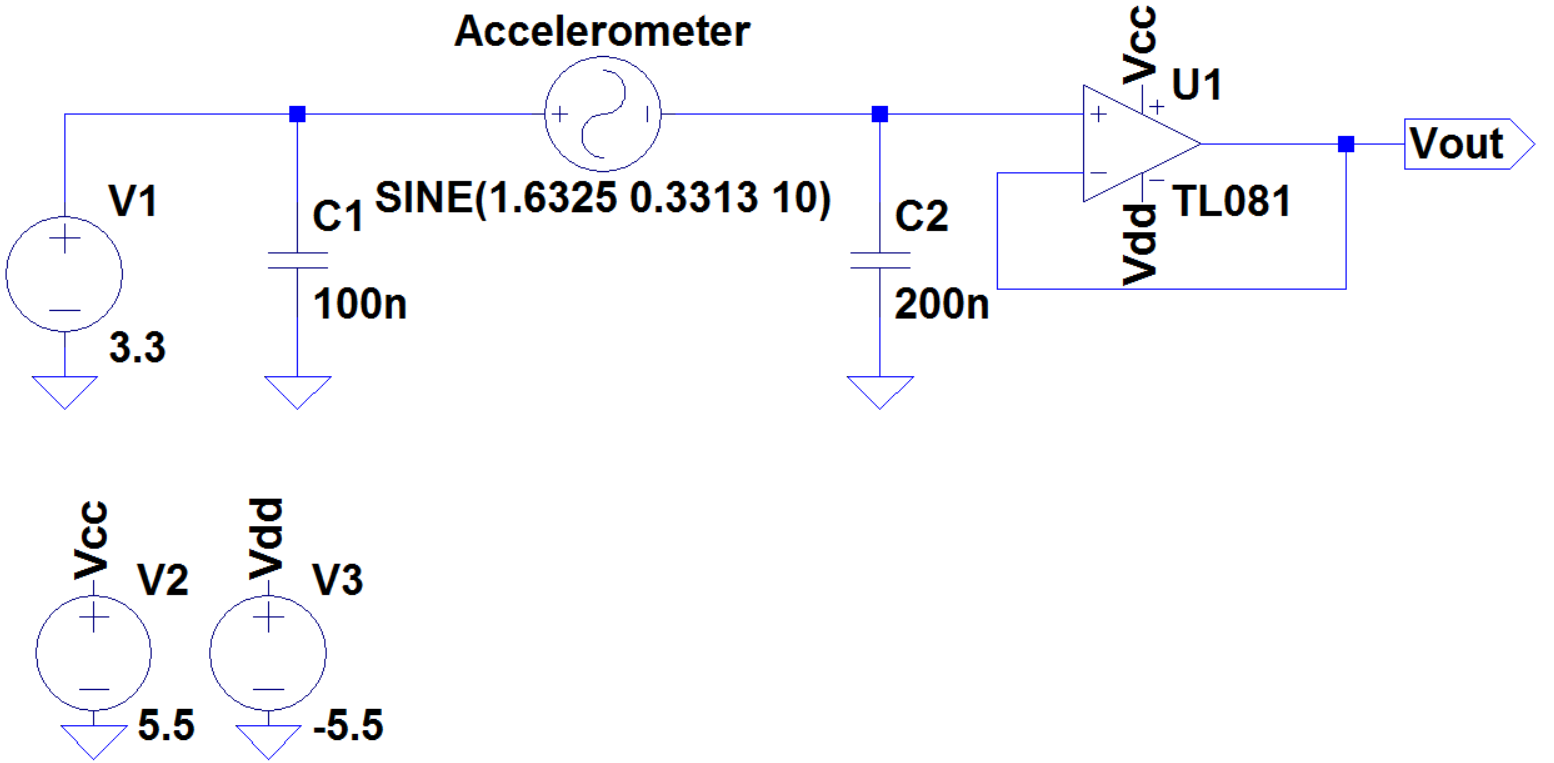
\includegraphics[scale=.4]{figures/cProblemloesning/Acc_Simulering1.PNG}
	\caption{På figuren ses designet af accelerometerblokken i LTspice. Accerometeret er symboliseret med en sinuskurve med et DC offset svarende til den tilførte strømforsyning fratrukket offsettet fra accelerometeret ved $0$g påvirkning, altså $5.5$V - $1.6325$V $=$ $3.8675$V. Herved centreres sinussignalet omkring $1.6325$V. Derudover indstilles amplituden til accelerometerets sensitivitet $0.3313$V og frekvensen til $10$Hz.}
	\label{fig:acc_simulering}
\end{figure}
\begin{figure}[H]
	\centering
	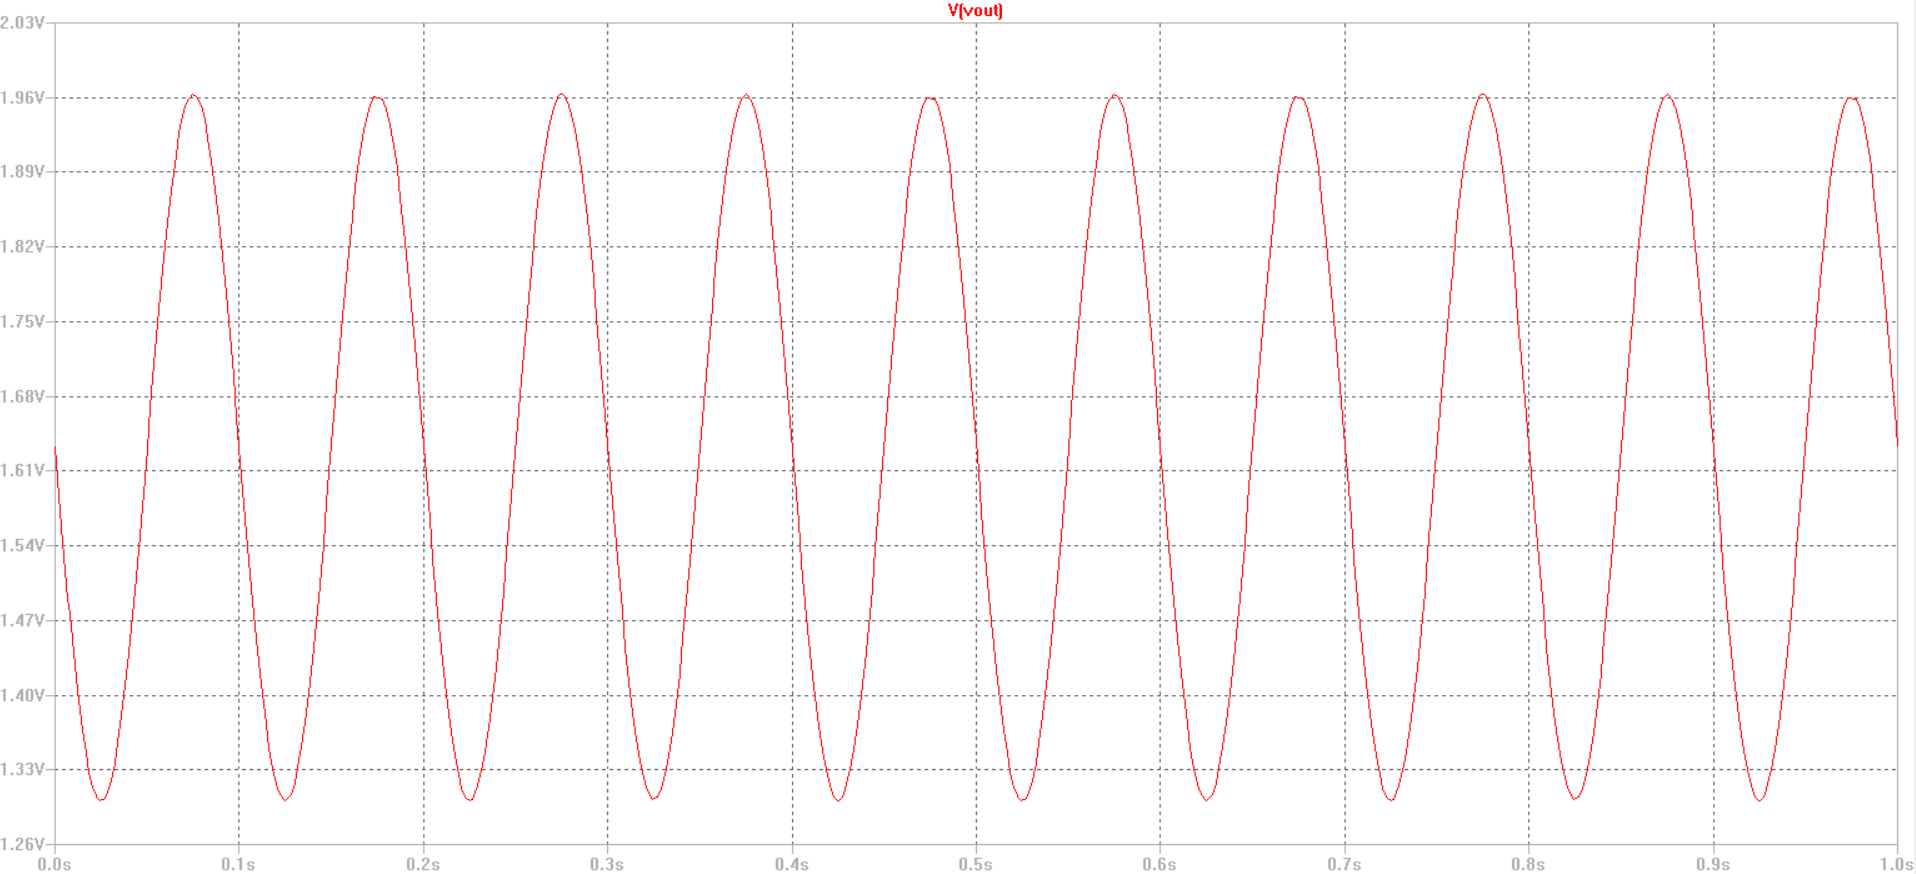
\includegraphics[scale=.35]{figures/cProblemloesning/Acc_Simulering2.PNG}
	\caption{På figuren ses simuleringen af accelerometret som en sinus med et offset på $1.6325$V, amplitude på $0.3313$V og frekvensen er $10$Hz. Der ses, at $V_{out}$ maksimalt er ca. $1.96$V og minimalt ca. $1.3$V.}
	\label{fig:acc_simulering_resultat}
\end{figure}

\subsubsection{Implementering og test}
I pilotforsøget blev der arbejdet med reelle komponenter, hvilket også blev benyttet til implementeringen. Derfor antages det, at der vil være en mindre afvigelse imellem resultaterne fra testen og pilotforsøget end imellem resultaterne fra testen og en eventuel simulering, da der i simuleringer arbejdes med ideelle komponenter. Accelerometerets båndbredde bestemmes af to $0.1\mu$F kapacitorer i parallelforbindelse, som derved vil give en samlet kapacitans på  $0.2\mu$F. De tre kapacitorer blev målt inden implementering samt den samlede kapacitans. Resultaterne fremgår i  \tableref{Tab:Acc_kondensator}:
\begin{table}[H]
	\centering
	\begin{tabular}{|l|l|l|l|}\hline
		& \textit{Teoretisk} & \textit{Målt} & \textit{\% afvigelse} \\ \hline
		\textit{C1}       & \textit{$0.1\mu$F} & $0.1004\mu$F  & $0.4\%$               \\ \hline		
		\textit{C2}       & \textit{$0.1\mu$F} & $0.1009\mu$F  & $0.9\%$               \\ \hline
		\textit{C3}       & \textit{$0.1\mu$F} & $0.0989\mu$F  & $1.1\%$               \\ \hline
		\textit{C2 || C3} & \textit{$0.2\mu$F} & $0.2002\mu$F  & $1\%$                \\ \hline
	\end{tabular}
	\caption{I tabellen ses det, at de tre kondensatorer afviger lidt fra deres teoretiske værdi, hvilket er forventet af reelle komponenter. Disse afvigelser vil derfor have en effekt på parallel forbindelsen imellem $C2$ og $C3$.}
	\label{Tab:Acc_kondensator}
\end{table}
\noindent Til opsamling af data fra accelerometret blev der benyttet et multimeter. I testen blev der foretaget en aflæsning med multimetret for $\pm8^\circ$ og $\pm13^\circ$. Disse fire værdier ses i \tableref{Tab:Acc_test_procent}. Den teoretiske stigning af volt pr. grad for henholdsvis negativ og positiv hældning er udregnet i bilag \ref{Bilag:Pilotforsoeg} på side \pageref{Bilag:Pilotforsoeg}. De teoretiske værdier for $8^\circ$ og $13^\circ$ udregnet derfor ud fra disse værdier. Dette gøres i følgende ligninger:
\begin{align}
(-0.0036 \cdot 13) + 1.6325 = 1.5858\text{V} \\
(-0.0036 \cdot 8) + 1.6325 = 1.6038\text{V}  \\
(0.0037 \cdot 8) + 1.6325 = 1.6619\text{V}  \\
(0.0037 \cdot 13) + 1.6325 = 1.6803\text{V}
\end{align}
Disse værdier indsættes og der udregnes en afvigelse.
\begin{table}[H]
	\centering
	\begin{tabular}{|l|l|l|l|}
		\hline
		\textit{\begin{tabular}[c]{@{}l@{}}Vinkel af\\ accelerometer\end{tabular}} &  \textit{\textit{\begin{tabular}[c]{@{}l@{}}Beregnet\\ Output\end{tabular}}} & \textit{Output} & \textit{\begin{tabular}[c]{@{}l@{}}\% afvigelse\\ ift. dektering\\ af hældningsgrad\end{tabular}} \\ \hline
%		$-90^\circ$     & $1.3092$V    & $\times$     & $\times$      \\ \hline
		\textit{$-13^\circ$}     & $1.5858$V    & $1.5686$V  & 1.08\%      \\ \hline
		\textit{$-8^\circ$}      & $1.6038$V    & $1.5947$V  & 0.57\%      \\ \hline
%		$0^\circ$       & $1.6325$V    & $\times$     & $\times$      \\ \hline
		\textit{$8^\circ$}       & $1.6619$V    & $1.6761$V  & 0.85\%      \\ \hline
		\textit{$13^\circ$}      & $1.6803$V    & $1.7114$V  & 1.85\%      \\ \hline
%		$90^\circ$      & $1.9638$V    & $\times$     & $\times$      \\ \hline
	\end{tabular}
	\caption{I tabellen ses det målte output fra bufferen ved en bestemt grad. Herved kan der beregnes en afvigelse i procent for accelerometerets afvigelse i detektion af grader.}
	\label{Tab:Acc_test_procent}
\end{table}
\noindent Der ses i tabel \tableref{Tab:Acc_test_procent}, at accelerometret har en maksimal afvigelse i detektionen af hældningsgrad på $1.85\%$. Derved overholder accelerometret tolerancerne, som er blevet stillet i afsnit \ref{OpsamlingsAfs} på side \pageref{OpsamlingsAfs} og accelerometret accepteres derfor.